\section{Dynamic Resource Allocation in a Manycore OS}\label{eval-dynamic}
%	c.	Dynamic System
%		i.	Single Application � right sizing
%			1.	Without phase changes
%			2.	With phase changes
%			3.	Baseline � all allocations
%			4.	Measure Energy
%		ii.	Video, Animation, and Throughput Applications w/o phase changes
%			1.	Show throughput and missed deadlines for all the possible mixes
%			2.	Is it possible to show optimal?
%			3.	What is the baseline?
%		iii.	Video, Animation, and Throughput Applications w/ phase changes
%			1.	Show throughput and missed deadlines for all the possible mixes
%			2.	Basically just to show the system works



\begin{figure*}[!t]
	\begin{center}	
		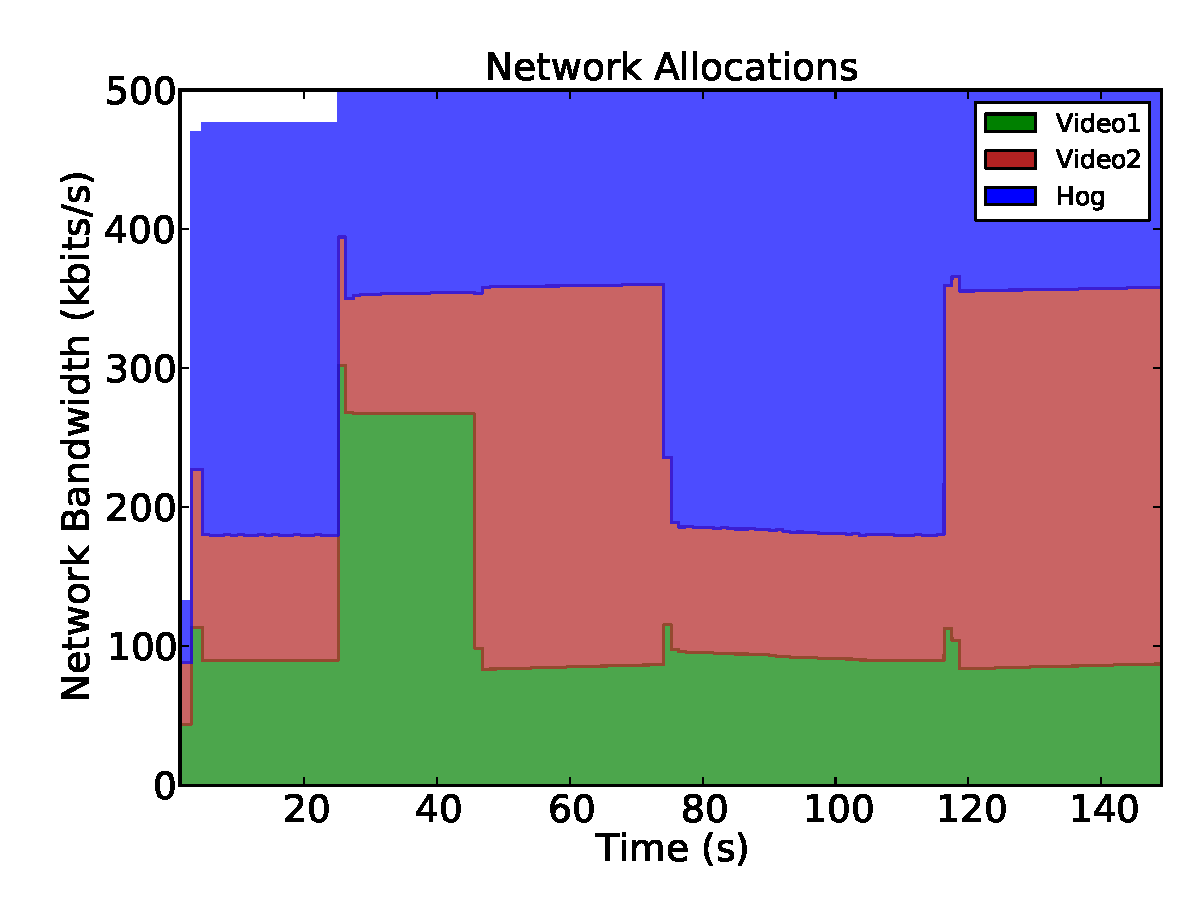
\includegraphics[bb=0 0 576 432,width=.49\textwidth]{dyn-alloc-wp-ns.pdf}
		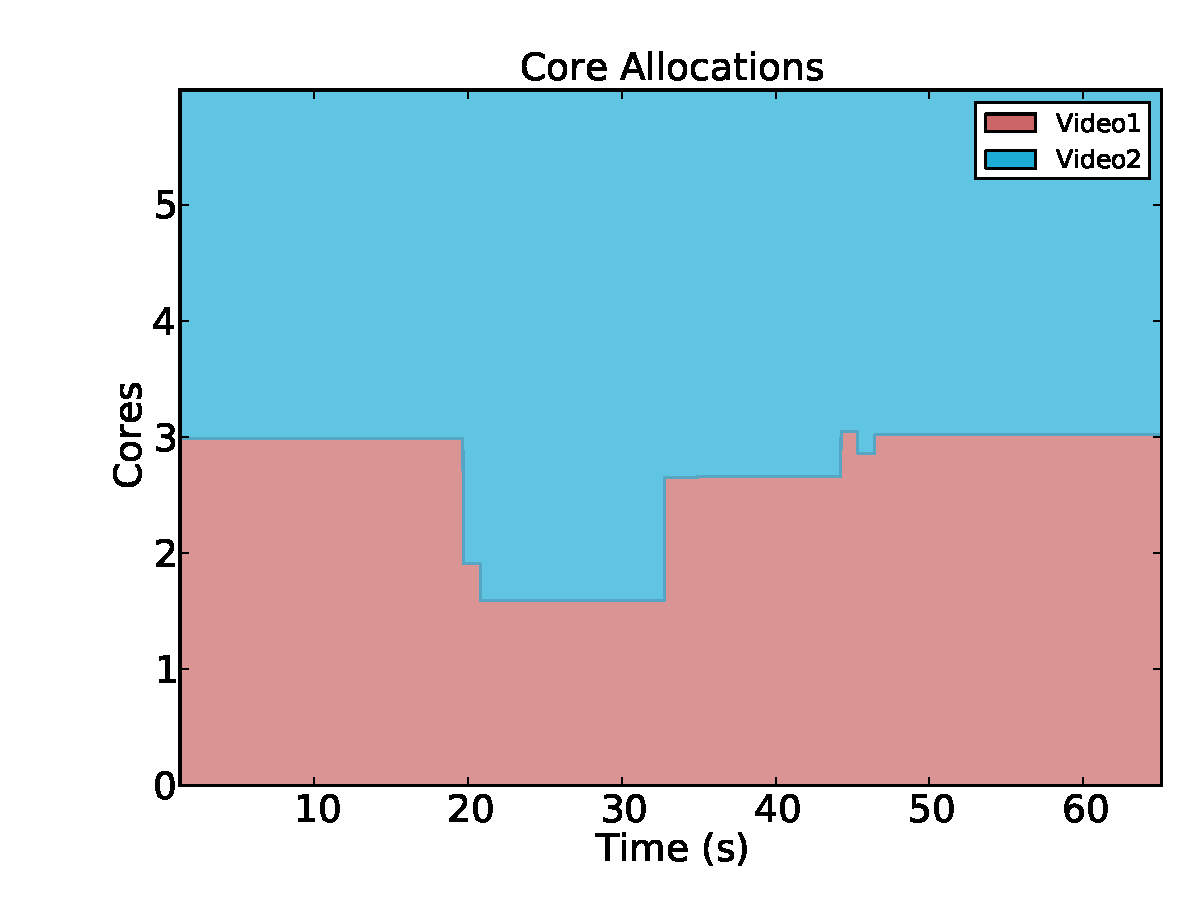
\includegraphics[bb=0 0 576 432,width=.49\textwidth]{dyn-alloc-wp-core.pdf}
		\caption{Wall Power Mode: Resource Allocations of video conferencing through time as the videos change resolution to adjust for which person is speaking. Hog represents as background task uploading files.}
		\label{video_experiment_wp}
	\end{center}
\end{figure*}

\begin{figure}[!t]
	\begin{center}	
		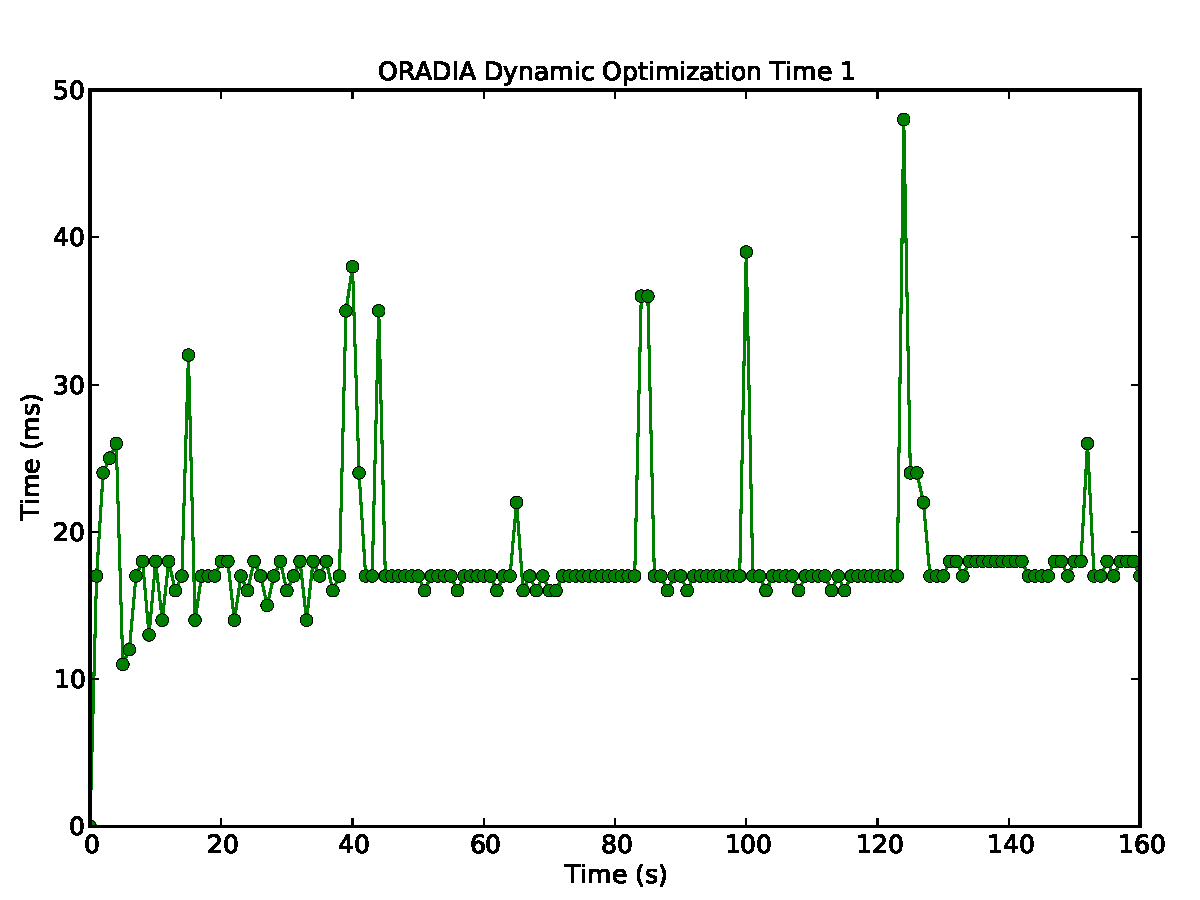
\includegraphics[bb=0 0 576 432,width=\columnwidth]{opt_time.pdf}
%		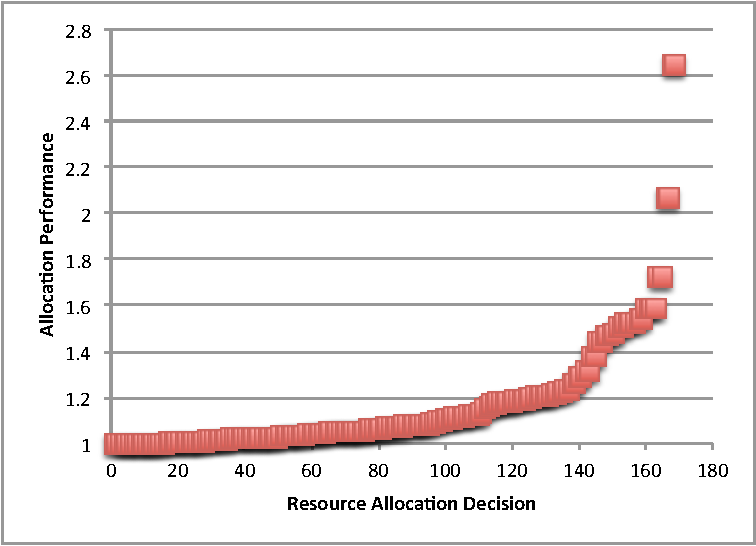
\includegraphics[width=.45\textwidth]{parsec_decision_points.pdf}
		\caption{Performance of our penalty optimization algorithm}
		\label{optimization_perf}
	\end{center}
\end{figure}

\begin{figure}[!t]
	\begin{center}	
		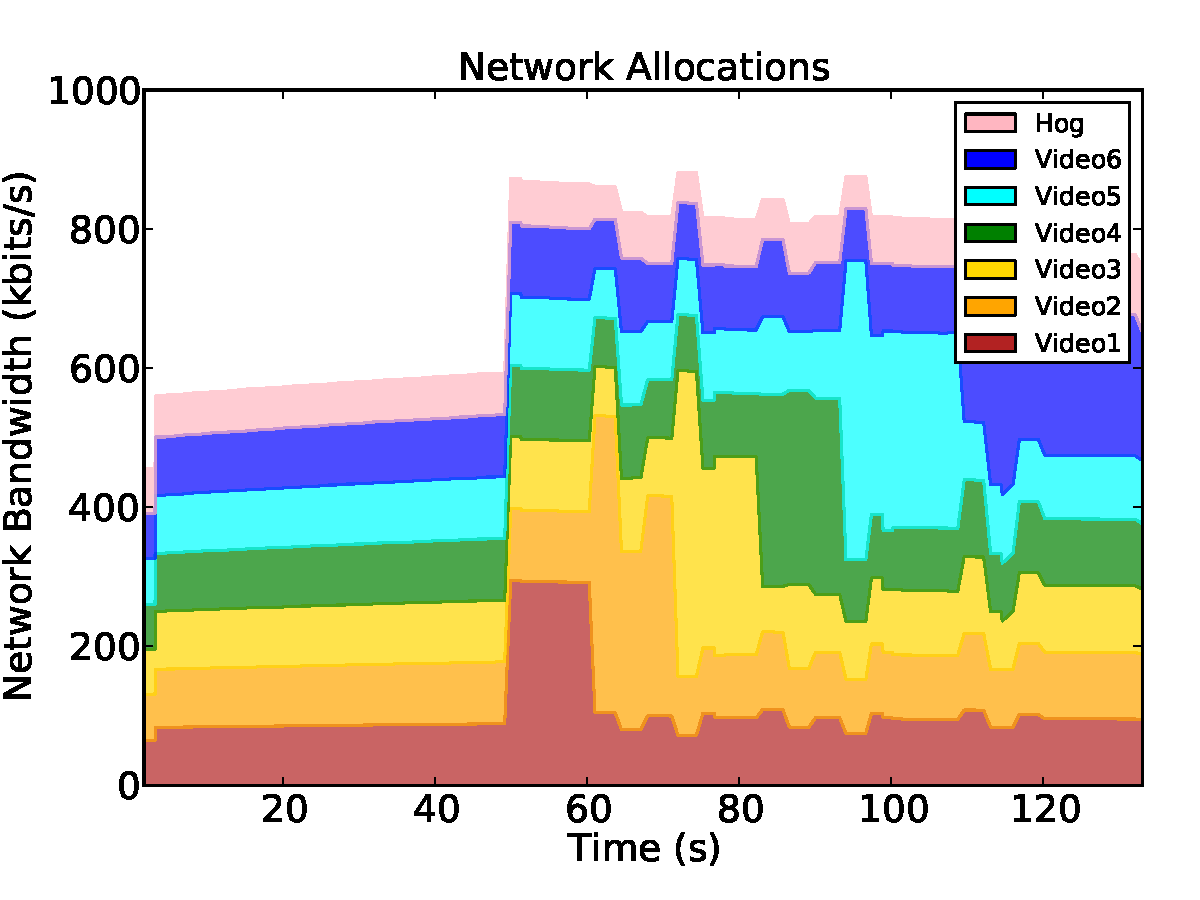
\includegraphics[bb=0 0 576 432,width=\columnwidth]{dyn-alloc-battery-ns.pdf}
		\caption{Battery Power Mode: Resource Allocations of video conferencing through time as the videos change resolution to adjust for which person is speaking. Hog represents as background task uploading files.}
		\label{video_experiment_battery}
	\end{center}
\end{figure}

%\cite{tess09,tess_dac}

To evaluate \pacora's ability to make real-time decisions in a real operating system, we implemented it in an in-house research operating system, \tess. We chose to implement in \tess rather than Linux for three reasons:
 \begin{itemize}\itemsep0pt \parskip0pt \parsep5pt
\item \tess separates resource allocation from scheduling so it more accurately reflects the system design \pacora assumes
\item \tess allows resource revocation, enabling \pacora to dynamically reallocate resources
\item \tess implements additional resource partitioning and QoS mechanisms, letting \pacora explore allocating more resource types
\end{itemize}
This dynamic framework is used to test our implementations of the algorithms, measure the overhead and reaction times, and illustrate \pacora's ability to work in a real system.

\subsection{Platform}
Our dynamic experiments are all run on an Intel Nehalem-EP system with two 2.66-GHz Xeon X5550 quad-core processors and hyperthreading enabled with 16 hardware threads. Tis system also contains a 1-Gbps Intel Pro/1000 Ethernet network adapter.
\tess allocates resources directly to applications, and the applications employ a second-level scheduler to schedule work onto the resources.  
%There are two scheduling frameworks available in \tess: a cooperative framework called Lithe (LIquid THrEads)~\cite{lithe} and a preemptive one called PULSE (Preemptive User-Level SchEduling).  
All of our experiments use a preemptive scheduling framework called PULSE (Preemptive User-Level SchEduling), with two different scheduling strategies: applications with responsiveness requirements use an earliest-deadline-first (EDF) scheduler and throughput-oriented applications use a global-round-robin (GRR) scheduler.

In addition to allocating cores and cache ways as with our static framework, \tess can also allocate fractions of network bandwidth.  In our experiments, we show \pacora allocating cores and network bandwidth because the experimental platform, which has the advantage of more cores, does not have cache partitioning.  We have also experimented with additional resources such as memory pages and cpu utilization, but the results are not presented here.

\subsection{Performance and Energy Measurement}
Applications report their own measured response times to \pacora through a message-passing interface built into \tess.  \pacora uses this information to build models, and we also use this information to show if the application is making its deadlines for the experiments.

\tess enables \pacora to directly measure the system energy.  However, energy counters are not available on our Nehalem-EP system and thus we extend the power model from the Sandy Bridge system to function as our Application 0 RTF.

\subsection{Description of Workloads}
Our workload is designed to represent the scenario of a video conference with participants from many remote locations.  There is a separate, performance guaranteed incoming video stream for each participant.
%New participants may join the conference and others may leave, increasing or decreasing the number of streams running at any given time.
The application adjusts video sizes based on which person is speaking. The speaker's video is larger and has higher resolution than the other video streams, and as the speaker changes the requirements for the video streams change. While conferencing, network-intensive tasks such as uploading and downloading files are executed in the background.
%While conferencing, compute-intensive tasks such as virus scans or file indexing could be executed in the background.

Our streaming video application is a multi-threaded, CPU- and network-intensive workload intended to simulate video chat applications like Skype and Facetime.
Each video stream is encoded offline in the H.264 format using libx264, transported across the network through a TCP connection from a Linux E5-based server, and decoded and displayed by the \tess client. The client receives, decodes, and displays each frame using libffmpeg and libx264. Each video stream has a corresponding EDF-scheduled thread with 33 ms deadlines using our second-level EDF scheduler.

%We use psearchy~\cite{psearchy}, a parallel text indexer, from MOSBENCH\cite{mosbench} as our file indexing application.

We also use a network bandwidth hog application designed represent an application like Google Drive or Dropbox uploading files to the cloud. The hog contends with the video player for bandwidth by constantly sending UDP messages to the Linux server.

\subsection{Resource Allocation Experiments}

We constrain the available resources in the system for \pacora to 1 Mbit/s network bandwidth and 6 cores to simulate a resource constrained system as this is a more challenging resource allocation problem.

In our experiment the video conference contains 6 incoming video streams.  At first no one is speaking and thus all the videos are small.  The person speaking changes from incoming videos 1- 6 in order with the videos resizing around every 10 seconds. We set the deadline to be 33 ms to represent a frame rate of 30 frames/sec. As this rate, small videos require 80 to 87 kbits/s depending on the particular frames. Large videos require 250 to 270 kbits/s.  We assign a moderate penalty (10.0) for missing the deadline to small videos, and a significant penalty (50.0) for the large videos.  We assign a small penalty for the network hog (1.0) with no deadline.

Figure~\ref{video_experiment_wp} shows the resource allocations for our video conference scenario when the computer is using ``wall power''.  We mean wall power to imply that saving power is less critical and thus we assign a low penalty slope to application 0.  \pacora gives 90 kbits/s to small videos, 280 kbit/s to large videos, and the remaining bandwidth is given to the network hog.  Video resizes can be seen as the ``steps'' in the graph: for example, Video1 becomes large at 24 seconds resulting in its allocation increasing from 90 kbits/s to 280 kbits/s.  Video2 becomes large at 33 seconds and Video1 returns to its original size.

We can see intermediate resource allocations (the ``columns'' in the graph) as \pacora transitions for one set of allocations to another.  The amount of intermediate resource allocations is controllable based on the exit conditions of the optimization algorithm.  If run much longer (50 ms), \pacora can completely eliminate the intermediate allocations, which may be appropriate in environments where resource reallocation is expensive and allocations do not need to be adapted frequently.  It is also possible provide guaranteed optimization times of around 20 $\micro$s, but at the cost of many more intermediate reallocations.  These results can be found in~\cite{pacora_tr}.

We choose this particular point in the space because we believed it strikes the right balance between reactivity and reallocation amounts for a client operating system. Figure~\ref{optimization_perf} shows the runtime of the optimization algorithm as it makes resource allocation decisions for the video scenario. The algorithm runs in 50 $\micro$s on average, with more significant reallocations taking from 250-350 $\micro$s.  Significant changes result in 1-2 intermediate reallocations.   In \tess, network bandwidth is easily reallocated and thus intermediate reallocations do not have much overhead.  Core allocations are also easily adjusted between fractional core amounts.

Core allocations are also shown in Figure~\ref{video_experiment_wp}.  Neither application in our scenario can take advantage of additional compute power thus each optimization results in the same core allocations for the applications regardless of video size.

Figure~\ref{video_experiment_battery} shows same scenario except the computer is now using ``battery power'' and thus we have increased the importance of application 0 (penalty 2.0).  The video applications are still allocated the necessary amount of resources for each video size.  However, the allocation of the network hog is significantly reduced to less than 70 kbits/s, and the remaining resources are left idle.








